\chapter{Aplicaciones continuas} \justifying
Sean $(X, \mc T_X)$ e $(Y, \mc T_Y)$ dos espacios topol\'ogicos.
\begin{defi}
    Una aplicaci\'on de conjuntos $f: X\longrightarrow Y$ es \textbf{continua} (como espacios topol\'ogicos) si se verifica que $f^*(\mc T_Y) \subseteq \mc T_X$ siendo $f^* : \mc P(Y) \longrightarrow \mc P(X)$. 
\end{defi}
\begin{obs}
    Esta definci\'on es equivalente a decir que para $V \in \mc T_Y$ abierto, entonces $f^*(V) = f^{-1}(V) \in \mc T_X$. Es decir, que la antiimagen por $f$ de cualquier abierto de $Y$ es abierto en $X$. 
\end{obs}
\begin{prop}
    Se verifica que las siguientes condiciones son equivalentes:
    \begin{enumerate}
        \item $f$ es continua ($f^{-1}(V)$ es abierto en $X$, para todo $V\subset Y$  abierto). 
        \item $f^{-1}(C)$ es cerrado en $X$ para todo cerrado $C\subset Y$.
        \item Para todo $x\in X$, y todo entorno $W$ de $f(x)$ en $Y$, $f^{-1}(W)$ es entorno de $x$ en $X$. (No se puede hacer sobre $Y$ porque no se tienen puntos sobre los que hacer entorno en $X$).
        \item Si $\mc B$ es una base de la topolog\'ia por abiertos de $Y$, $f^{-1}(B) $ es abierto en $X$ para todo $B \in \mc B$. 
        \item Si $\mc B$ es base de cerrados de la topolog\'ia en $Y$, $f^{-1}(B)$ es cerrado en $X$ para todo $B\in \mc B$.
        \item Si $\{\mc B(y)\}_{y \in Y}$ es una base de entornos de la topolog\'ia de $Y$ entonces $f^{-1}(B)$ es entorno de $x$ para todo $B \in \mc B(f(x))$ y $\forall \, x \in X$.  
    \end{enumerate}
\end{prop}
\begin{dem}
    $1)\Rightarrow 2)$ $\forall \, Z \subset Y$ subconjunto, $f^{-1}(Y-Z) = X-f^{-1}(Z)$. 

    $1)\Rightarrow 3)$ Sea $W$ entorno de $f(x)\subset Y$. Por tanto, existe $V$ abierto en $Y$ tal que $f(x) \in V \subset W$, por lo que 
    $$x\in f^{-1}(f(x)) \subset f^{-1}(V) \subset f^{-1}(W)$$
    donde $f^{-1}(V)$ abierto de $X$ por la condici\'on 1) y entorno de $x$, como quer\'iamos ver.
    
    $3) \Rightarrow 1)$ Sea $V \subset Y$ abierto, veamos que $f^{-1}(V) \subset X$ es abierto. Veamos para ello que $\forall \, x\in f^{-1}(V), \, f^{-1}(V)$ es entorno de $x$. 

    $V$ es abierto de $Y$ y $f(x) \in V \Rightarrow V$ es entorno de $f(x)$, y $f^{-1}(V)$ es entorno del punto $x$. 
    
    $1) \Rightarrow 4)$

    $4) \Rightarrow 1)$ Sea $V \subset Y$ abierto $\Rightarrow V = \displaystyle \bigcup_{\overset{i\in I}{B_i \in \mc B} \, } B_i \Rightarrow f^{-1}(V) = \bigcup f^{-1}(B_i)$ siendo $f^{-1}(V) $ y $f^{-1}(B_i)$ abiertos. Si $\mc B$ es una base de la topolog\'ia por abiertos de $Y$, $f^{-1}(B)$ es abierto en $X$ para todo $B\in \mc B$. 
    
    $2) \iff 5)$ De la misma forma con intersecciones. 

    $3) \iff 6)$ \textcolor{red}{Terminar}
\end{dem}
\begin{defi}
    Una aplicaci\'on continua es \textbf{inyectiva} o \textbf{epiyectiva} si lo es como aplicaci\'on de conjuntos.

    Una aplicaci\'on continua es \textbf{isomorfismo de espacios topológicos} (\textbf{homeomorfismo}) si es biyectiva si lo es como aplicaci\'on de conjuntos y $f^{-1}: Y \longrightarrow X$ es continua.
\end{defi}
\begin{ejem}
    \begin{itemize} 
        \item Dado un espacio topológico $(X,\mc T_X)$
        $$\bt (X, \mc T_X) \rar{\text{Id}_X} & (X, \mc T_X) \\[-5mm] x \rarmaps & x \et$$
        es un homeomorfismo
        \item Sea $X$ un conjunto
        $$\bt (X, \mc T_{dis}) \rar{\text{Id}_X} & (X, \mc T_{triv}) \\[-5mm] x \rarmaps & x \et$$
        es continua y biyectiva, pero la inversa 
        $$\bt (X, \mc T_{triv}) \rar{\text{Id}_X^{-1}} & (X, \mc T_{dis}) \\[-5mm] x \rarmaps & x \et$$
        no es continua pues para la antiimagen de un abierto de la discreta no podemos asegurar que sea abierto de la trivial, pues no tiene m\'as abiertos que $X$ y $\emptyset$. Esto nos dice que los homeomorfismos nos dan equivalencias entre las topologías de espacios. 
    \end{itemize}
\end{ejem}
\begin{prop}
    Sean $(X, \mc T_X)$ e $(Y, \mc T_Y)$ espacios topol\'ogicos y $f: (X, \mc T_X) \longrightarrow(Y, \mc T_Y)$ una aplicaci\'on continua. Sea $\mc T_X'$ y $\mc T_Y'$ otras topolog\'ias en $X$ e $Y$ respectivamente tales que $\mc T_X \subseteq \mc T_X'$, $\mc T_Y' \subseteq \mc T_Y$, entonces
    $$\bt f : (X, \mc T_X') \rar & (Y, \mc T_Y') \et \text{ es continua}$$
\end{prop}
\begin{dem}
    Como para todo abierto de $Y$ queremos que su antiimagen sea abierto en $X$, si tenemos una topolog\'ia m\'as pequeña en $Y$ es m\'as f\'acil que sea continua, y si en $X$ tenemos una topolog\'ia m\'as grande, es m\'as f\'acil a\'un que sea abierto, luego continua. \textcolor{red}{Formalizar}. 
\end{dem}
\begin{obs}
    Las aplicaciones constantes son continuas. Sea $y_o \in Y$, 
    $$\bt f_{y_o}: X \rar & Y \\[-5mm] \, \, x \rarmaps & y_o \et$$
    Si $V\subset Y$ es abierto,
    $$f^{-1}(V) = \begin{cases}
        X & \text{ si } y_o \in V \\ \emptyset & \text{ si } y_o \nin V
    \end{cases}$$
\end{obs}

\begin{prop}
Sea $f: X \longrightarrow Y$ una aplicación.
\begin{enumerate}
    \item Sea $(X, \mc T_X)$ un espacio topológico. Se verifica que para todo espacio topológico $(Y, \mc T_Y)$ y toda aplicación de conjuntos $f: X \longrightarrow Y$, esta es continua $\iff \mc T_X = \mc T_{\text{disc}}$ (máxima topología que se puede poner).
    \item Sea $(Y, \mc T_Y)$ un espacio topológico. Se verifica que para todo espacio topológico $(X, \mc T_X)$ y toda aplicación de conjuntos $f: X \longrightarrow Y$, esta es continua $\iff \mc T_Y = \mc T_i$ (mínima topología que se pueda poner en un espacio/conjunto).
\end{enumerate}
\end{prop}

\begin{dem}\begin{enumerate}
    \item $\Leftarrow)$ Si $\mc T_X = \mc T_{\text{disc}} \implies f: (X, \mc T_{\text{disc}}) \longrightarrow (Y, \mc T_Y)$ es continua, pues para todo abierto $V \in \mc T_Y$ se cumple $f^{-1}(V) \subseteq \mathcal{P}(X) = \mc T_{\text{disc}}$.
        
    $\Rightarrow)$ Sea $(X, \mc T_{\text{disc}}) = (Y, \mc T_Y)$.
        
        Tomamos $f = \text{Id}_X: (X, \mc T_X) \longrightarrow (X, \mc T_{\text{disc}})$, que por hipótesis debe ser continua.
        \[
            \begin{array}{ccc}
            A & \reflectbox{$\mapsto$} & \text{Id}_X^{-1}(A) = A \\
            \text{ab.} & & \text{ab.}
            \end{array}
        \]
        Como es continua, dado $A \in \mc T_{\text{disc}}$, $\text{Id}_X^{-1}(A) = A$ es abierto también en $(X, \mc T_X)$, luego $\mc T_{\text{disc}} \subseteq \mc T_X$. Como $\mc T_{\text{disc}}$ es la topología más grande, $\mc T_X \subseteq \mc T_{\text{disc}} \implies \mc T_X = \mc T_{\text{disc}}$.
    \item $\Leftarrow)$ Si $\mc T_Y = \mc T_i = \{\emptyset, Y\}$, para cualquier abierto $V \in \mc T_Y$, su preimagen es $f^{-1}(\emptyset) = \emptyset \in \mc T_X$ o $f^{-1}(Y) = X \in \mc T_X$, por lo que $f$ siempre es continua.

        $\Rightarrow)$  Supongamos que la condición se cumple para todo espacio topológico $(X, \mc T_X)$ y toda aplicación $f$. Tomamos $(X, \mc T_X) = (Y, \mc T_i)$ con la topología indiscreta y la aplicación identidad $f = \text{Id}_Y: (Y, \mc T_i) \longrightarrow (Y, \mc T_Y)$. Por hipótesis, esta identidad debe ser continua. Dado cualquier abierto $V \in \mc T_Y$, la preimagen $\text{Id}_Y^{-1}(V) = V$ debe ser un abierto en $(Y, \mc T_i) = \{\emptyset, Y\}$. Por lo tanto, necesariamente $V = \emptyset$ o $V = Y$, concluyendo que $\mc T_Y = \mc T_i$.
\end{enumerate}
\end{dem}

\begin{ejem}
En $(\mathbb{R}, \mc T_u)$:
\[
    [0, 1] \simeq [a, b] \quad \text{con } a < b
\]
\[
    (0, 1) \simeq (a, b) \quad \text{homeomorfos}
\] Estiramos el intervalo $[0, 1]$ con una homotecia multiplicando por $(b - a)$:
$$ \bt 
    \left[0, 1\right] \rar{h_{(b-a)}} & \left[0, b - a\right] \\[-5mm] 
    z \rarmaps & (b - a)z &[-13mm]  \text{continua (lo sabemos)} \\[-5mm] 
    \frac{1}{b - a} w & \arrow[mapsto]{l} w &[-13mm]  \text{la inversa es otra homotecia (continua)}
    \et $$
Luego es un homeomorfismo porque ambas homotecias tienen inversa y su inversa (otra homotecia) es continua. Ahora hacemos una traslación:
$$ \bt
    \left[0, b-a\right] \rar{T_a} & \left[a, b\right] \\[-5mm] 
    w \rarmaps & w + a & \text{continua} \\[-5mm]
    z - a & \arrow[mapsto]{l} z & \text{continua}
    \et $$

Luego:
\[
    [0, 1] \xrightarrow[\sim]{h_{b-a}} [0, b-a] \xrightarrow[\sim]{T_a} [a, b]
\]
\end{ejem}
\begin{ejem}[$(\mathbb{R}, \mc T_u)$]
Estirar un intervalo abierto hasta (cubrir) $\mathbb{R}$ también es homeomorfismo:
\[
    (a, b) \simeq \mathbb{R}
\]

Tomamos la semicircunferencia centrada en $(0,2)$, $SC_{(0,2)}$.

Como una circunferencia centrada en ese punto sería $\mathcal{C}_{(0,2)} \equiv x^2 + (y-2)^2 = 1$, la ecuación de la semicircunferencia es:
\[
    SC_{(0,2)} \equiv x^2 + (y-2)^2 = 1 \quad \text{con } 1 \le y < 2 \quad \subseteq (\mathbb{R}^2, \mc T_u).
\]

Ahora queremos proyectar esa semicircunferencia al intervalo $(-1, 1)$. Consideramos la aplicación:
$$\bt
    SC_{(0,2)}  \rar{\sim} & (-1, 1) \simeq  (a, b) \\[-5mm]
    (x, y)  \rarmaps & x &[-13mm] \text{continua} \\[-5mm]
    \left(z, 2 - \sqrt{1 - z^2}\right) & \arrow[mapsto]{l} z &[-13mm] \text{continua} &[-13mm] & \text{(todas las operaciones son continuas)}
   \et $$

Por tanto, esta aplicación es un homeomorfismo. Al final, solo estamos ``aplastando una circunferencia''. Como $(-1, 1)$ es homeomorfo a cualquier intervalo $(a, b)$, ya que hemos visto que $(-1, 1) \simeq (a, b)$.

Ahora vemos que $SC_{(0,2)} \simeq \mathbb{R}$. Tomamos la aplicación que consiste en unir cualquier punto de la circunferencia con el $(0, 2)$ y cortar esa recta con el eje $\mathbb{R}$ ($y = 0$).

La recta que une cualquier punto $(x_0, y_0)$ de la circunferencia con $(0, 2)$ es:
\[r \equiv y - 2 = \frac{y_0 - 2}{x_0} x.\]

Queremos cortar con la recta $s \equiv y = 0$. Luego el punto resultante es $\left(x = \frac{-2x_0}{y_0 - 2}, 0\right)$.

Es decir, definimos la aplicación:
$$\bt SC_{(0,2)} = (a,b) \rar{\sim} & \mathbb{R} \\ (x_0, y_0) \rarmaps & \frac{-2x_0}{y_0 - 2} &[-10mm] \text{continua} \\ \left( \pm \frac{2}{\sqrt{4 + z_0^2}}, \frac{2z_0^2}{4 + z_0^2} + 2 \right) & \arrow[mapsto]{l} z_0 & \text{continua} \et$$
Por tanto, $(a, b) \simeq \mathbb{R}$ homeomorfo.
\end{ejem}
\begin{ejer}
Demostrar que $\mathcal{C}_{(0,0)} \setminus \{N\} \simeq \mathbb{R} \simeq SC_{(0,0)}$. Siendo $N$ el punto $(0, a)$ tal que $a$ es el máximo o el mínimo valor que toma el eje vertical en la esfera/circunferencia.

La ecuación de la circunferencia es $x^2 + y^2 = b$.
$$\bt \mathcal{C}_{(0,0)} \setminus \{N\} \rar{\sim} & \mathbb{R} \\ (x_0, y_0) \rarmaps & \dots \et$$
\begin{center}
\begin{tikzpicture}[scale=1.6, >=stealth]
    % Radio de la circunferencia
    \def\R{1.3}
    
    % Coordenadas clave
    \coordinate (O) at (0,0);
    \coordinate (N) at (0,\R);
    \coordinate (S) at (0,-\R);
    
    % Circunferencia centrada en el origen
    \draw[thick] (O) circle (\R cm);
    
    % Ejes principales (cruzan completamente)
    \draw (-2.3, 0) -- (2.3, 0); % Eje horizontal (R)
    \draw (0, -1.7) -- (0, 1.7); % Eje vertical (N - S)
    
    % -------------------------------------------------------------
    % RECTA DERECHA: Pasa por N(0, R) y por un punto P_right de la circunferencia
    % Ángulo de P_right = 35° => P_right = (R*cos(35°), R*sin(35°))
    % Intersección exacta con el eje y = 0: x = R * cos(35°) / (1 - sin(35°))
    % -------------------------------------------------------------
    \coordinate (Pright) at ({ \R*cos(35) }, { \R*sin(35) });
    \coordinate (Xright) at ({ \R*cos(35)/(1 - sin(35)) }, 0);
    
    % Dibujamos la recta prolongada
    \draw ($(N)!-0.15!(Xright)$) -- ($(N)!1.1!(Xright)$);
    
    % -------------------------------------------------------------
    % RECTA IZQUIERDA: Pasa por N(0, R) y corta al eje horizontal en x_left < 0
    % Tomamos el corte en x = -0.8
    % Intersección con la circunferencia: ángulo = -118.07° aprox.
    % -------------------------------------------------------------
    \coordinate (Xleft) at (-0.8, 0);
    \coordinate (Pleft) at ({ -2*\R*\R*(-0.8) / ((-0.8)*(-0.8) + \R*\R) }, { \R*( (-0.8)*(-0.8) - \R*\R ) / ((-0.8)*(-0.8) + \R*\R) });
    
    % Dibujamos la recta prolongada
    \draw ($(N)!-0.15!(Xleft)$) -- ($(N)!1.55!(Xleft)$);
    
    % -------------------------------------------------------------
    % PUNTOS Y ETIQUETAS
    % -------------------------------------------------------------
    \filldraw (N) circle (1.2pt) node[above right] {$N$};
    \filldraw (S) circle (1.2pt) node[below right] {$S$};
    \filldraw (O) circle (1pt) node[below right] {$(0,0)$};
    
    % Puntos sobre la recta derecha
    \filldraw (Pright) circle (1.2pt);
    \filldraw (Xright) circle (1.2pt);
    
    % Puntos sobre la recta izquierda
    \filldraw (Xleft) circle (1.2pt);
    \filldraw (Pleft) circle (1.2pt);
\end{tikzpicture}
\end{center}
\end{ejer}

\begin{ejer}
Sea $X$ un espacio topológico. $A \subseteq X$ es subespacio topológico $\iff (A, \mc T_X\vert{}_A)$.
$$\bt (A, \mc T_X\vert{}_A) \rar[hook]{i_A} & (X, \mc T_X) \\ a \rarmaps & a & [-12mm] \text{continua} \et$$
$i_A$ es continua porque $i_A^*(\mc T_X) = \mc T_X\vert{}_A$.
\end{ejer}
\noindent \textbf{Nota}.  Para definir aplicaciones, primero mira una aplicación entre conjuntos y luego comprueba si es continua.

\begin{propis}[de las aplicaciones continuas] \, 
\begin{enumerate}
    \item Si $X, Y, Z$ son espacios topol\'ogicos y $f: X \longrightarrow Y$, $g:Y \longrightarrow Z$ son aplicaciones continuas, entonces $g \circ f : X \longrightarrow Z$ es continua.
    \item Si $f: X \longrightarrow Y$ es continua y $A \subset X$ es subespacio topol\'ogico, entonces 
    $$\bt f\vert{}_A : A \rar & Y  \\ a \rarmaps & f\vert{}_A(x) \coloneqq f(x) \et$$
    es continua.
    \item Si $f: X \longrightarrow Y$ es continua y $B\subset Y$ subespacio topol\'ogico con $\Im \, f\subset B$, entonces 
    $$\bt f^B: X \rar & B \\ x \rarmaps & f(x) \et$$
    es continua.
    \item Sea $f: X\longrightarrow Z$ aplicaci\'on continua con $Z \subset Y$ subespacio topol\'ogico, entonces 
    $$\bt f^Y: X \rar & Y \\ x \rarmaps & f(x) \et$$
    es continua.
    \item Si $\{U_i\}_{i \in I}$ es un recubrimiento por abiertos de $X$ ($X = \bigcup U_i$), y sea $f: X \longrightarrow Y$ una aplicaci\'on de conjuntos tal que $f\vert{}_{U_i} : U_i \longrightarrow Y$ es continua para todo $i\in I$ (equivalentemente diremos que la continuidad de una aplicaci\'on es un concepto local). 
\end{enumerate}
\end{propis}
\begin{dem}\,gracias a que  
    \begin{enumerate}
        \item Sea $W\subset Z$ un abierto,veamos que $(g\circ f)^{-1}(W) \subset X$ es abierto. 
        
        Como $(g\circ f)^{-1}(W) = f^{-1}(g^{-1}(W))$ y $g$ es continua, $g^{-1}(W) \subset Y$ es abierto, de forma que como $f$ tambi\'en es continua y $V = g^{-1}(W) \subset Y$ es abierto, $f^{-1}(V) = f^{-1}(g^{-1}(W))$ es abierto en $X$, como quer\'iamos demostrar. 
        
        \noindent \textbf{Observaci\'on:} $(g\circ f)^{-1}(W) \neq (f^{-1} \circ g^{-1})(W)$ pues $f^{-1}$ y $g^{-1}$ NO existen como aplicaci\'on. 

        \item $\bt A \rar[hook]{i_A} & X \rar{f} & Y \et$ de forma que $f\vert{}_A = f\circ i_A$ composici\'on de aplicaciones continuas, por 1., continua. 
        
        \item Sea $W \subset B$ un abierto de $B$, por lo que por ser la topolog\'ia inducida en $Y$, existe $U\subset Y$ abierto de $Y$ tal que $V \cap B = W$. Entonces $f^{-1}(V) \subset X$ es abierto por ser $f$ continua, pero $f^{-1}(V)  = f^{-1}(V \cap \Im f) = f^{-1}(V \cap B) = f^{-1}(W)=(f^B)^{-1}(W)$ poque $\Im f\subset B$.  
        \item Similar a 3.
        \item Sea $V\subset Y$ abierto y veamos que $f^{-1}(V)$ es abierto. $f^{-1}(V) \subset X$ luego
        $$f^{-1}(V) = f^{-1}(V) \cap X = f^{-1}(V) \cap \left( \bigcup_{i \in I} U_i \right) = \bigcup_{i\in I} \left(f^{-1}(V) \cap U \right) = \bigcup_{i \in I} f\vert{}_{U_i}^{-1}(V)$$
        por ser $f\vert{}_{U_i} ^{-1}(V)$ abierto en $U_i$ (que es abierto), son abiertos en $X$ $\forall \, i$, la uni\'on arbitraria de abiertos es abierto y por tanto $f^{-1}(V)$ es abierto como quer\'iamos demostrar. 
    \end{enumerate}
\end{dem}
\begin{defi}
    Una apliaci\'on de conjuntos $f : X\longrightarrow Y$ entre espacios topol\'ogicos, entonces se dice que $f$ es \textbf{continua en un punto $x\in X$} si para todo entorno $V$ de $f(x)$, $f^{-1}(V)$ es entorno de $x$ en $X$. 

    Se verifica que $f$ es continua si y solo si $f$ es continua en todos los puntos de $X$. 
\end{defi}
Sea $f: X\longrightarrow Y$ aplicaci\'on continua
\begin{propis}
[NO] Si $V \subset Y$ es abierto $\Rightarrow$ $f^{-1}(V)$ es abierto en $X$. Su rec\'iproco es falso, si $V\subset Y$ es un subconjunto tal que $f^{-1}(V) \subset X$ es abierto $\not\Rightarrow V \subset Y$ sea abierto. Por $\text{Id}: (X, \mc T_{dis}) \longrightarrow (X, \mc T_{triv})$ que es continua se demuestra. 

Sea $U\subset X$ abierto $\not\Rightarrow f(U)$ es abierto en $Y$. 
$$\bt \bb R \rar{f} & \bb R \\ x \rarmaps & x^2 \\ (-2,2) \rarmaps & \left[0,4\right) \et$$
de forma que la imagen de un abierto $(-2,2)$ no es abierto $[0,4)$
\end{propis}
\begin{defi}
    Una aplicaci\'on de conjuntos $f : X \longrightarrow Y$ entre espacios topol\'ogicos es \textbf{abierta} si para todo abierto $U$ de $X$, $f(U)$ es abierto en $Y$ (no suponer que $f$ sea continua).
\end{defi}
\begin{ejem}
    $\text{Id}: (X, \mc T_{triv}) \longrightarrow (X, \mc T_{dis})$ es abierta pero no continua.
\end{ejem}
\begin{defi}
Una aplicaci\'on de conjuntos $f : X \longrightarrow Y$ entre espacios topol\'ogicos es \textbf{cerrada} si para todo cerrado $C$ de $X$, $f(C)$ es cerrado en $Y$ (no suponer que $f$ sea continua).
\end{defi}
\begin{ejer}
    Sea $X$ un espacio topol\'ogico y $A\subset X$ un subespacio topol\'ogico, $i_A: A \hookrightarrow X$ es continua. Se verifica que 
    \begin{itemize}
        \item $i_A$ es abierta $\iff \, A \subset X$ es abierto
        \item $i_A$ es cerrada $\iff \, A \subset X$ es cerrada. 
    \end{itemize}    
\end{ejer}

\begin{ejer}
    Aplicaci\'on abierta $\not\Rightarrow$ cerrada. 
\end{ejer}
\begin{sol}
    No, porque el complementario no funciona bien con la imagen. Sea $C = X-U, \, f(C) = f(X-U) \neq Y - f(U)$ (con la antiimagen s\'i).
\end{sol}

Sea $f: X \longrightarrow Y$ una aplicaci\'on continua
\begin{defi}
    Decimos que $f$ es una \textbf{inmersión topológica} si $f$ establece un homeomorfismo 
    $$\bt f: X \rar{\sim} & (\Im f, \mc T_Y \vert{} _{\Im f}) \et \Rightarrow \bt f: X \arrow[swap]{rd}{\sim} \rar[hook] & Y \\[-5mm] & \Im f \arrow[phantom]{u}{\cup}  \et \text{ es inyectiva.}$$
    (No es que sean homeomorfos, es a trav\'es de $f$) ($X$ se identifica con el subespacio topol\'ogico imagen)
\end{defi}
\begin{ejem}
    Si $X$ es espacio topol\'ogico, $A \subset X$, 
    $$\bt (A, \mc T_X\vert{}_A) \arrow[swap]{rd}{\Id_A} \rar[hook]{i_A} & (X, \mc T_X) \\  & (\Im i_A = A, \mc T_X \vert{} _A) \et$$
\end{ejem}
\begin{defi}
    Una \textbf{función de $X$} es una aplicaci\'on $f: X\longrightarrow \bb Q$ \'o $f: X\longrightarrow \bb C \simeq \bb R^2$
\end{defi}

\section{Topolog\'ia inicial}
\begin{custom}
[Motivaci\'on] Si $f: X \longrightarrow Y$ es una aplicaci\'on continua, 
$$\bt f^* : \mc P(Y) \rar & \mc P(X) \\[-5mm] \mc T_Y \rarmaps & f^*(\mc T_Y) \subset \mc T_X \et$$
$f^*(\mc T_Y)$ es la topolog\'ia menos fina (m\'as pequeña) en $X$ que hace a $f$ continua (si tenemos otra topolog\'ia que no la contenga, $f$ no es continua). 
\end{custom}
Sea $(Y, \mc T_Y)$ un espacio topol\'ogico, $X$ un conjunto y $f:X \longrightarrow Y$ una aplicaci\'on de conjuntos
\begin{defi}
    Se define la \textbf{topología inicial de la aplicación $f$} como la topolog\'ia en $X$ dada por 
    $$\bt f^* : \mc P(Y) \rar & \mc P(X) \\[-5mm] \mc T_Y \rarmaps & f^*(\mc T_Y)  \et$$
    Es la topolog\'ia menos fina que en $X$ que hace a la aplicaci\'on de conjuntos $f: X\longrightarrow Y$ continua
    $$f^*(\mc T_Y) \equiv \mc T_f = \{U \subset X : \text{ existe } V \text{ abierto en } Y \text{ tal que } f^*(V) = f^{-1}(V) = U\}$$
\end{defi}\begin{ejem}
    $X, \mc T_X$ espacio topol\'ogico y $A \subset X$ un subconjunto, para $i_A: A \hookrightarrow X$ se tiene que 
    $$\mc T_{i_A} = i_A^*(\mc T_X) = \mc T_X\vert{}_A$$
\end{ejem}

Sean $\{(X_i, \mc T_{Y_i})\}_{i \in I}$ espacios topol\'ogicos, $X$ un conjunto y $\{f_i : X \longrightarrow Y_i\}_{i \in I}$ aplicaciones de conjuntos
\begin{defi}
    La \textbf{topología inicial en $X$ de las aplicaciones $\{f_i\}_{i \in I}$}, denotada por $\mc T_{\{f_i\}_{i \in I}}$, es la topolog\'ia menos fina en $X$ que hace que todas las aplicaciones de conjuntos $f_i: X \longrightarrow Y_i$ sea continuas $\forall \, i \in I$
    $$\bt f^*_i : \mc P(Y_i) \rar & \mc P(X) \\[-5mm] \mc T_{Y_i} \rarmaps & f^*(\mc T_{Y_i}) = \mc T_{f_i} \et \Rightarrow   \, \, \mc T_{f_i} \text{ tiene que contener a todas las topolog\'ias } \{f^*_i(\mc T_{Y_i})\}$$
    (ver el subconjunto m\'as pequeño de $\mc P(X)$ que las contiene).
\end{defi} 
\begin{obs}
    $\displaystyle \bigcup_{i \in I} f_i^*(\mc T_{Y_i}) \subset \mc P(X)$ no tiene por qu\'e ser topolog\'ia, pues la uni\'on arbitraria no lo asegura. La intersecci\'on s\'i.

    Buscamos la menor topolog\'ia que lo contenga. No es topolog\'ia ni base, pero es subbase de una topolog\'ia. 

    En efecto, sea $x\in X, \, i \in I, Y_i \in \mc T_{Y_i}, \, X\in f_i^*(Y_i) \in \bigcup f_i^*(\mc T_{Y_i})$, $f_i^*(Y_i) = f_i^{-1}(Y_i)=X$.

    La menor topolog\'ia que la contiene es la generada por esa sub-base 
    $$S\mc B_{\{f_i\}} = \bigcup_{i \in I} f_i^*(\mc T_{Y_i}) = \{ U \subset X : \text{ para alg\'un } i \in I, \, U \in f_i^*(\mc T_{Y_i}) \equiv \text{ existe } V_i \in \mc T_{Y_i} \text{ tal que } f_i^{-1}(V_i) = U\}$$

    Consideremos $\mc B_{\{f_i\}}$ la base generada por $S\mc B_{\{f_i\}}$
    $$\mc B_{\{f_i\}} = \{f_{i_1}^{-1}(V_{i_1}) \cap \cdots \cap f_{i_r}^{-1}(V_{i_r}) \text{ con } i_1, \ldots, i_r \in I, \, V_{i_j} \subset Y_{i_j}\text{ abierto para cada } j \in \{i_1, \ldots, i_r\}\}$$

    La topolog\'ia 
    $$\mc T_{\{F_i\}} \equiv \left\{ \text{topolog\'ia generada por } \mc B^{\{f_i\}} \right\} = \left\{\bigcup_{\underset{i_1, \ldots, i_r \in I}{\, \forall \, r \in \bb N}} f^{-1}_{i_1}(V_{i_1}) \cap \cdots \cap f^{-1}_{i_r}(V_{i_r})\right\}$$
    es la uni\'on arbitraria de intersecciones finitas de antiim\'agenes de abiertos, que ahora s\'i podemos asegurar que sea una toolog\'ia. 
\end{obs}

\medskip

Sean $\{f_i : X\longrightarrow (Y_i, \mc T_{Y_i})\}_{i \in I}$ aplicaciones de conjuntos.
\begin{propi}
    [Universal de la Topolog\'ia inicial] La topolog\'ia inicial de las aplicaciones $\{f_i\}_{i \in I}, \, \mc T_{\{f_i\}}$ en $X$ es la \'unica topolog\'ia de $X$ que verifica que para todo espacio topol\'ogico $(Z, \mc T_Z)$ y toda aplicaci\'on $g: Z \longrightarrow X$
    $$g \text{ es continua con  } (X, \mc T_{\{f_i\}}) \iff f_i \circ g: Z \longrightarrow Y_i \text{ es continua } \forall i \in I$$
\end{propi}
\begin{dem}
$\Rightarrow)$ $g$ es continua y $f_i$ tambi\'en para todo $i\in I$ por la topolog\'ia inicial, por lo que  
$$\bt Z \rar{g} \arrow[bend right=10mm,swap]{rr}{f_i \circ g} & X \rar{f_i} & Y_i \et$$
como la composici\'on de aplicaciones continuas es continua, aseguramos que $g\circ f_i$ es continua.

$\Leftarrow)$ Supongamos que $f_i \circ g$ es continua $\forall i \in I$.

Para comprobar que $g$ es continua, basta comrpobar que $g^{-1}(f_i^{-1}(U_i)) \subset Z$ es abierto para cada $i \in I$ y para cada $V_i \subset Y_i$
$$Z \subset g^{-1}(f_i^{-1}(V_i)) = (\underbrace{f_i \circ g}_{\text{continua}})^{-1}(V_i) $$
asegurando as\'i que es un abierto en $Z$.
\end{dem}

\medskip

\begin{prop}
Sea $X$ un conjunto, $\{ (Y_i, \mc T_{Y_i}) \}_{i \in I}$ una familia de espacios topológicos y $\{f_i \colon X \longrightarrow Y_i\}_{i \in I}$ una familia de aplicaciones. Si $\mc T_X$ es una topología en $X$ que satisface la propiedad universal de la topología inicial, entonces:
\[
    \mc T_X = \mc T_{\{f_i\}}
\]
\end{prop}

\begin{dem}
Las aplicaciones $f_i \colon (X, \mc T_X) \longrightarrow (Y_i, \mc T_{Y_i})$ son continuas para todo $i \in I$. En efecto, al considerar la aplicación identidad $\operatorname{Id}_X \colon (X, \mc T_X) \longrightarrow (X, \mc T_X)$, se tiene 
\[
\bt (X, \mc T_X) \rar{\operatorname{Id}_X} \arrow[bend right=10mm]{rr}{f_i} & (X, \mc T_X) \rar{f_i} & Y_i \et
\]
Dado que $\operatorname{Id}_X$ es continua, la composición $f_i = f_i \circ \operatorname{Id}_X$ es continua. Por la definición de topología inicial (al ser la menos fina que hace continuas a las $f_i$), se deduce que
\[
    \mc T_{\{f_i\}} \subseteq \mc T_X.
\]

Recíprocamente, por la propiedad universal de la topología inicial $\mc T_{\{f_i\}}$, la aplicación identidad $\operatorname{Id}_X \colon (X, \mc T_X) \longrightarrow (X, \mc T_{\{f_i\}})$ es continua si y solo si lo es la composición
\[
\bt (X, \mc T_X) \rar{\operatorname{Id}_X} \arrow[bend right=10mm]{rr}{f_i} & (X, \mc T_X) \rar{f_i} & Y_i \et
\]
Como las aplicaciones $f_i$ son continuas por hipótesis sobre $\mc T_X$, se deduce que $\operatorname{Id}_X \colon (X, \mc T_X) \longrightarrow (X, \mc T_{\{f_i\}})$ es continua. Por tanto
\[
    \mc T_X \subseteq \mc T_{\{f_i\}}.
\]

Concluimos que $\mc T_X = \mc T_{\{f_i\}}$.
\end{dem}

\section{Producto directo de espacios topol\'ogicos}

Sean $\{(X_i,\mc T_i)\}_{i\in I}$  una familia de espacios topol\'ogicos. Sea $\{X_i\}_{i \in I}$ una familia de conjuntos, se tiene el conjunto
$$\prod_{i\in I} X_i = \left\{ (x_i)_{i\in I} : x_i \in X_i \right\}$$
Para cada $j\in I$, se tiene la aplicaci\'on de conjuntos
$$\bt \pi_j : \displaystyle \prod_{i \in I} X_i \rar & X_j \\[-5mm] (x_i)_{i\in I} \rarmaps & x_j \et$$

Sea $\mc T_{\{\pi_j\}_{j \in I}}$ la topolog\'ia inicial en $\prod_{i \in I} X_i$ de las proyecciones can\'onicas $\{\pi_j: \prod_{i \in I} X_i \longrightarrow X_j\}_{j \in I}$, la llamamos topolog\'ia del producto directo, $\mc T_{\pi}$ en $\prod_{i \in I} X_i$.

El espacio topol\'ogico producto directo de espacio topol\'ogicos $\{(X_i, \mc T_i)\}_{i\in I}$ es por definici\'on $\left(\prod_{i \in I} X_i, \mc T_{\pi} \right)$

\section{Base de la topología producto directo ($\tau_\pi$)}

Dada una familia de espacios topológicos $\{(X_i, \tau_{X_i})\}_{i \in I}$, un elemento de la base de la topología inicial por las proyecciones canónicas $\pi_i \colon \prod_{i \in I} X_i \longrightarrow X_i$ viene dado por la intersección finita de antiimágenes de abiertos:
\[
    \pi_{i_1}^{-1}(U_{i_1}) \cap \cdots \cap \pi_{i_r}^{-1}(U_{i_r}) = V \quad (\text{elemento de la base de la topología producto directo}).
\]

\paragraph{Caso de dos factores ($I = \{1, 2\}$):}
Consideremos $I = \{1, 2\}$. Se tiene que
\[
    \pi_1^{-1}(U_1) \cap \pi_2^{-1}(U_2) = \textcolor{green}{U_1 \times U_2}.
\] por la siguiente figura podemos observarlo

\begin{center}
\begin{tikzpicture}[scale=1]
    % Ejes
    \draw[thick, ->] (-0.5,0) -- (4.5,0) node[below right] {$X_1$};
    \draw[thick, ->] (0,-0.5) -- (0,3.5) node[above left] {$X_2$};

    % Intervalo U1 en X1
    \draw[very thick, blue] (1.2,0) -- (2.8,0);
    \node[blue, below] at (2, -0.1) {$U_1$};
    \draw[blue] (1.2,0.1) -- (1.2,-0.1);
    \draw[blue] (2.8,0.1) -- (2.8,-0.1);

    % Intervalo U2 en X2
    \draw[very thick, red] (0,1.5) -- (0,2.5);
    \node[red, left] at (-0.1, 2) {$U_2$};
    \draw[red] (0.1,1.5) -- (-0.1,1.5);
    \draw[red] (0.1,2.5) -- (-0.1,2.5);

    % Lineas discontinuas de proyeccion
    \draw[dashed, blue] (1.2,-1) -- (1.2,4);
    \draw[dashed, blue] (2.8,-1) -- (2.8,4);
    \draw[dashed, red] (-1,1.5) -- (4,1.5);
    \draw[dashed, red] (-1,2.5) -- (4,2.5);

    % Rectangulo producto U1 x U2 rayado
    \fill[pattern=north east lines, pattern color=green!70] (1.2,1.5) rectangle (2.8,2.5);
    \draw[thick] (1.2,1.5) rectangle (2.8,2.5);

    % Flechas de proyeccion y etiquetas
    %\node at (2, 2.9) {$X_1 \times X_2$};
    \draw[<-, thick, blue] (3.1,0.5) -- (3.1, 1.8) node[above] {$\pi_1$};
    \draw[<-, thick, red] (0.5,2.8) -- (2,2.8) node[right] {$\pi_2$};
    \node[blue] at (2,3.8)  {$\pi_1^{-1}(U_1)$};
    \node[red] at (4.7, 2) {$\pi_2^{-1}(U_2)$};
\end{tikzpicture}
\end{center}
de forma que 
\[
    \pi_1^{-1}(U_1) = U_1 \times X_2 \subseteq X_1 \times X_2, \qquad \pi_2^{-1}(U_2) = X_1 \times U_2 \subseteq X_1 \times X_2.
\]

Caso finito ($I = \{1, \ldots, n\}$):
Si $U_1 \subseteq X_1, \ldots, U_n \subseteq X_n$, la topología coincide con la topología de las cajas:
\[
    \tau_\pi = \tau_{\text{cajas}} = \left\langle \{U_1 \times \cdots \times U_n \mid U_i \subseteq X_i \text{ abiertos}\} \right\rangle.
\]

Caso arbitrario: Para un índice $i_1 \in I$ cualquiera
\[
    \pi_{i_1}^{-1}(U_{i_1}) = U_{i_1} \times \prod_{j \neq i_1} X_j = \left\{ (x_i)_{i \in I} \in \prod_{i \in I} X_i \;\middle|\; x_{i_1} \in U_{i_1} \right\}.
\]
Para un número finito de índices $\{i_1, \ldots, i_r\} \subseteq I$
\[
    \pi_{i_1}^{-1}(U_{i_1}) \cap \cdots \cap \pi_{i_r}^{-1}(U_{i_r}) = U_{i_1} \times \cdots \times U_{i_r} \times \prod_{j \notin \{i_1, \ldots, i_r\}} X_j.
\]
En cambio, la \textbf{topología de las cajas} sobre un producto arbitrario se define como:
\[
    \tau_{\text{cajas}} = \left\langle \left\{ \prod_{i \in I} U_i \;\middle|\; U_i \subseteq X_i \text{ abiertos} \right\} \right\rangle.
\]

En general, para productos infinitos se verifica que $\tau_\pi \subsetneq \tau_{\text{cajas}}$.
\begin{custom}
    [Contraejemplo] $\prod_{n \in \bb N} \bb R = \bb R^{\bb N}$. Sus elementos son $(x_n)_{n \in \bb N}: x_n \in \bb R$, es decir, una sucesi\'on, por lo que $\bb R^{\bb N}$ es el espacio de sucesiones de n\'umeros reales. De esta forma, se tiene que $(\bb R^{\bb N}, \mc T_{\pi})$ y $(\bb R^{\bb N}, \mc T_{cajas})$, se tiene la aplicaci\'on de conjuntos,
    $$\bt \bb R \rar{c} & \bb R^{\bb N} \\[-5mm] \lambda \rarmaps & (\lambda)_{n\in\bb N}\et$$
     de forma que $c$ es continua en $(\bb R, \mc T_d)\longrightarrow (\bb R^{\bb N}, \mc T_{\pi})$ pero no en $(\bb R, \mc T_d)\longrightarrow (\bb R^{\bb N}, \mc T_{cajas})$.

     En efecto, por la propiedad universal, 
     $$\bt \bb R \rar{c} \arrow[bend left=10mm]{rr}{\text{Id}_X} & \bb R^{\bb N} \rar{\pi_n} & \bb R \\[-5mm] 
     \lambda \rarmaps & (\lambda)_{n \in \bb N} \rarmaps & \lambda
     \et$$ de forma que como $\pi_n$ es continua, $\text{Id}_X$ es continua, entonces $c$ es continua.

     Por otro lado, sea 
     $$\bb R^{\bb N} \supset U := (-1,1) \times (-\nicefrac{1}{2}, \nicefrac{1}{2}) \times \cdots \times (-\nicefrac{1}{n}, \nicefrac{1}{n}) \times \cdots $$
     es un abierto b\'asico en $\mc T_{cajas}$ por ser producto de abiertos, y al hacerle antiimagen por $c$, $\lambda \in (-\nicefrac{1}{n}, \nicefrac{1}{n})\forall n\in \bb N$, por lo que tiene que pertenecer a su intersecci\'on,  
     $$c^{-1} (U) = \bigcap_{n \in \bb N} (-\nicefrac{1}{n}, \nicefrac{1}{n}) = \{0\} \in \bb R$$
     que no es abierto, por lo que $c$ no es continua.
\end{custom}
\begin{ejer}
    Sea $X_i$ espacios topol\'ogicos y $f:X\longrightarrow Y$ aplicaci\'on continua e inyectiva. $f$ es inmersi\'on topol\'ogica si y solo si $\mc T_X = \mc T_f =$ topolog\'ia inicial de $f$. 
    
    (Falta comprobar que $f^{-1}$ sea continua sobre $\Im f$. Por ser $f$ continua, $\mc T_f \subset \mc T_X$, hay que comprobar la inclusi\'on contraria). 
\end{ejer}
\begin{ejer}
    Sea $X$ espacio topol\'ogico y $f,g$ funciones continuas en $X$. Definimos
    $$\bt X \rar{f+g} & \bb R \\[-5mm] x \rarmaps & (f+g)(x) = f(x) + g(x) \et$$
    y si $f,g$ son continuas, entonces $f+g$ es continua. Podemos ver que 
    $$\bt X \rar{(f,g)} & \b R \times \bb R \rar{s} & \bb R \\[-5mm]
    x \rarmaps & (f(x),g(x)) \rarmaps & f(x)+g(x)
    \et$$
    de forma que $(f,g)$ es continua si y solo si las composiciones con $\pi_i$ lo son
    $$\bt & & \bb R \\[-5mm] X \arrow[bend left=8mm,swap]{rru}{g}  \arrow[bend right=8mm]{rrd}{f} \rar{(f,g)} & \bb R\times \bb R \arrow[swap]{ru}{\pi_1}\arrow{rd}{\pi_2} \\[-5mm] & & \bb R \et$$
    y como $f$ y $g$ son continuas y $\pi_i$ tambi\'en, $(f,g)$ tambi\'en, y la suma por tanto tambi\'en. De la misma forma, $f(x) \cdot g(x)$. 
\end{ejer}
\section{Topolog\'ia final}
\begin{custom}
    [Motivaci\'on] Sea $f: X \longrightarrow Y$ continua, tenemos $f^*: \mc P(Y) \longrightarrow \mc P(X)$ cumple que $f^*(\mc T_Y) \subset \mc T_X$. Pero es lo mismo que $\mc T_Y \subset (f^*)^{-1}(\mc T_X)$, esto es $(f^*)^{-1}(\mc T_X)$ es la topolog\'ia en $Y$ m\'as fina (m\'as grande, con m\'as abiertos) que hace a $f$ continua.
\end{custom}
Sea $(X, \mc T_X)$ espacio topol\'ogico, $Y$ un conjunto y $f: X \longrightarrow Y$ una aplicaci\'on de conjuntos. 
\begin{defi}
    La \textbf{topolog\'ia final} de $f$ es la topolog\'ia en $Y$ m\'as fina que hace a $f$ continua, y es $(f^*)^{-1}(\mc T_X) =: \mc T^f=\mc T_{f^*}$
    $$\mc T^f = \left\{ V \subset Y : f^*(V) \in \mc T_X  \right\} =  \left\{ V \subset Y : f^{-1}(V) \text{ es abierto en } X  \right\}$$
    (si $f$ es biyectiva es $\mc T_X$)
\end{defi}
\begin{ejer}
    Comprobar que $(f^*)^{-1}(\mc T_X)$ es topolog\'ia si $\mc T_X$ lo es.
\end{ejer}
\subsection{Caso general}
Sean $\{(X_i,\mc T_i)\}_{i \in I}$ espacios topol\'ogicos, $Y$ un conjunto, $\{f_i: X_i \longrightarrow Y\}_{i \in I}$
\begin{defi}
    La \textbf{topolog\'ia final} de las aplicaciones $\{f_i : X_i \longrightarrow Y\}_{i \in I}$ en $Y$ es la topolog\'ia m\'as fina en $Y$ que hace a todas las aplicaciones $\{f_i\}_{i \in I}$ continuas. (Cualquier topolog\'ia en $Y$ que haga a las $f_i$ continuas est\'a contenida en $\mc T^{\{f_i\}}$). 

    Para que $f_i: X_i \longrightarrow (Y, \mc T_i)$ sea continua $Y$ tiene que tener $\mc T^{f_i}$. Es decir, $\mc T_i \subset \mc T^{f_i}$. Entonces, para que todas sean continuas cada $\mc T^{f_i}$ tiene que estar contenidas, es decir, es
    $$\mc T^{\{f_i\}} = \bigcap_{i \in I} \mc T^{f_i} = \left\{ V \subset Y : f_i^{-1}(V) \subset X_i \text{ es abierto}, \forall \, i \in I \right\}$$
\end{defi}
\begin{ejer}
    Probar que $\bigcap_{i \in I} \mc T_i$ es topolog\'ia si las $\mc T_i$ lo son.
\end{ejer}
\begin{propi}
[Universal de la topolog\'ia final] Sean $\{(X_i,\mc T_i)\}_{i \in I}$ espacios topol\'ogicos, $Y$ un conjunto y $\{f_i : X_i \longrightarrow Y\}_{i \in I}$ aplicaciones. La topolog\'ia final $\mc T^{\{f_i\}}$ de las aplicaciones $\{f_i\}_{i \in I}$ es la \'unica topolog\'ia en $Y$ que verifica la siguiente propiedad:

Para todo espacio topol\'ogico $(Z, \mc T_Z)$ y para toda aplicaci\'on $g: Y \longrightarrow Z$ (de conjuntos),
$$g \text{ es continua } \iff  g\circ f_i \text{ son continuas } \forall \, i \in I, \bt X_i \arrow[bend right=10mm]{rr}{g\circ f_i} \rar{f_i} & Y \rar{g} & Z \et$$
\end{propi}
\begin{dem}
    $\Rightarrow)$ $Y \xrightarrow{g} Z$ continua, $X_i \xrightarrow{f_i} (Y, \mc T^{\{f_i\}})$ continuas $\forall \, i\in I$, 
    $$\bt X_i \rar{f_i} \arrow[bend right=10mm]{rr}{g\circ f_i}  & Y \rar{g} & Z \et \text{ es continua por ser composici\'on de continuas. }$$
    $\Leftarrow)$ Sea $W \subset Z$ abierto, veamos que $g^{-1}(W)$ es abierto en $ (Y, \mc T^{\{f_i\}})$.
    
    Por la definici\'on de la topolog\'ia final, $g^{-1}(W)$ es abierto en $ (Y, \mc T^{\{f_i\}}) \iff f_i^{-1}(g^{-1}(W)) \subset X_i$ es abierto $\forall \, i \in I$, pero 
    $$f_i^{-1}(g^{-1}(W)) = (g\circ f_i)^{-1}(W)$$
    y $g\circ f_i$ es continua por hip\'otesis $\forall \, i \in I$, por lo que $g^{-1}(W)$ es un abierto. 
\end{dem}
\section{Uni\'on disjunta}
Sean $\{X_i\}_{i\in I}$ conjuntos, se define la uniçón disjunta de conjuntos
$$\bigsqcup_{i \in I} X_i= \{(i, x_i) \, / \, x_i \in X_i, \, i \in I\}$$
que intuitivamente es ``dar un elemento de cada uno de los conjuntos''.
\begin{ejem}
    $\bb R \sqcup \bb R \ni (1,0) = O_1$ es el 0 de la primera copia de $\bb R$ y $(2,0)=O_2$ es el 0 de la segunda, de forma que todos los elementos est\'an repetidos, y gr\'aficamente son dos rectas que no tienen elementos comunes. 
\end{ejem}
\begin{ejem}
    Sean $A, B\subset X$ dos subconjuntos $A\cup B \subset X$ y $A\sqcup B$ son iguales si $A\cap B = \emptyset$. En caso contrario, si $A\cap B \neq \emptyset$,
    $$\bt A\sqcup B \rar & A\cup B \\[-5mm] (1,a) \rarmaps & a \\[-5mm] (2,b) \rarmaps & b \et$$
    es epiyectiva. Si $c\in A\cap B$, 
    $$\bt (1,c) \rarmaps & c \\[-5mm] (2,c) \arrow[mapsto]{ru} & \et$$
\end{ejem}
\begin{ejem}
    Sea $E$ espacio vectorial y $E_1, E_2 \subset E$ dos subespacios,
    $$\bt 0 \rar & E_1 \cap E_2 \rar & E_1 \oplus E_2 \rar & E_1+E_2 \rar & 0 \\[-5mm]
    & & (e_1,e_2) \rarmaps & e_1 + e_2 \rarmaps & 0 \\[-5mm] & e \rarmaps & (e,e)
    \et$$
    Aqu\'i la uni\'on disjunta es la suma directa de espacio vectoriales $\bigoplus_{i \in I} E_i \subset \prod_{i \in I} E_i$ est\'a contenido en el producto directo. 
\end{ejem}
Para cada $j \in I$, se tiene la inmersi\'on
$$\bt \varphi_j : X_j \rar[hook] & \bigsqcup X_i \\[-5mm] x_j \rarmaps & (j, x_j) \et$$
que es inyectiva.

\section{Topolog\'ia uni\'on disjunta}

Podemos dotar a la uni\'on disjunta de la topolog\'ia final de las inmersiones, es decir, dadas las inmersiones can\'onicas $\big\{ \varphi_j : X_j \hookrightarrow \bigsqcup_{i \in I} X_i \big\}_{j\in I}$ se tiene que $  \left( \underset{i \in I}{\bigsqcup} X_i, \mc T^{\{\varphi_j\}}\right)$ es el espacio topol\'ogico uni\'on disjunta. Tambi\'en se denota $\mc T^{\{\varphi_j\}} = \mc T_{\sqcup} = \mc T^{\sqcup}$ y se le llama topolog\'ia uni\'on disjunta, y es una topolog\'ia final.

¿Cu\'ando un subconjunto es abierto? Sea $W \subset \big(\bigsqcup X_i, \mc T_{\sqcup}\big)$ es abierto si $\varphi_j^{-1}(W)\subset X_j$ es abierto para cada $j\in I$, pero $$\varphi_j^{-1}(W) = W\cap X_j = \varphi_j^{-1}(W\cap \varphi(X_j))$$
pues la inversa de las inmersiones (que son inyectivas) es como cortar.

Sea $(Z, \mc T_Z)$ un espacio topol\'ogico y $\bigsqcup_j X_j \overset{g}{\longrightarrow} Z$,
$$ g \text{ es continua }\iff g\circ \varphi_j: X_i \longrightarrow Z \text{ es continua } \forall \, j \in I. $$
¡El espacio topológico unión disjunta es con esta topología en concreto!
\begin{ejem}
    $\{\bb R, \bb R\}$, $W\subset \bb R \sqcup \bb R$ es abierto $\iff$ $W \cap \bb R_1$ y $W\cap \bb R_2$ son abiertos en $\bb R$ ($\bb R_1$ es la primera copia de $\bb R$ y $\bb R_2$ la segunda). Además, $\bb R \sqcup \bb R\supset W = (W\cap \bb R_1) \sqcup (W\cap \bb R_2)$ es la uni\'on disjunta de abiertos.
\end{ejem}
Si $U_i \subset X_i$ es abierto, $W=\bigsqcup U_i \subset \left( \underset{i \in I}{\bigsqcup} X_i, \mc T_{\sqcup} \right)$ si $W\cap X_i = U_i$ (es obvio).
\section{Topolog\'ia cociente}
Sea $X$ un conjunto, $R$ una relaci\'on de equivalencia, $\modulo{X}{R} = \{[x]_R, \, x\in X\}$ es el conjunto cociente de $X$, por la relaci\'on $R$, que sabemos que es uni\'on disjunta de sus clases de equivalencia $[x]$. Además, se tiene la aplicación de paso al cociente
$$\bt \pi: X \rar & \modulo{X}{R} \\[-6mm] x \rarmaps & \left[x\right]_R  \et$$
que es epiyectiva.
\begin{defi}    
Se dice que un subconjunto $A \subseteq X$ es \textbf{saturado} para la relación $R$ si $\forall a \in A$, $[a]_R \subseteq A$, es decir, si $x R a \implies x \in A$.
\end{defi}
\begin{defi}    
Se define la \textbf{saturación} de un subconjunto $A \subseteq X$ por la relación $R$ como:
\[
    X \supseteq [A]_R = \bigcup_{a \in A} [a]_R \supseteq A
\]
es el menor subconjunto saturado que contiene a $A$. Esta uni\'on es disjunta pues las clases de equivalencia lo son.

Otra manera de ponerlo es $[A]_R = \pi^{-1}(\pi(A)) \supseteq A$.
\end{defi}
\begin{prop}
    Un conjunto es saturado $\iff A = [A]_R$.
\end{prop}

\subsection{Espacio topológico cociente}

Sea $R$ una relación de equivalencia en $X$, $X \xrightarrow{\pi} \modulo{X}{R} \quad \text{como conjuntos}$
\begin{defi}
La \textbf{topología cociente} en $\modulo{X}{R}$ es la topología final de la aplicación $\pi$ de paso al cociente, denotada por $\mathcal{T}_{{X}/{R}}$ y
\[
   \bt (X, \mathcal{T}_X) \rar{\pi} & \left(\modulo{X}{R}, \mathcal{T}_{X/R}\right) \et \quad \text{es continua}
\]

Un subconjunto $W \subseteq \left(\modulo{X}{R}, \mathcal{T}_{X/R}\right)$ es abierto (ó cerrado) $\iff \pi^{-1}(W)$ es abierto (ó cerrado) en $X$.

\end{defi}
\begin{prop}
    Se verifica que si todo abierto (ó cerrado) de $X$ es saturado por la relación $R$, entonces $\pi$ es una aplicación abierta (ó cerrada).
\end{prop}\begin{dem}
    
Sea $U \subseteq X$ abierto. ¿Es $\pi(U) \subseteq \modulo{X}{R}$ abierto?

Esto ocurre $\iff \pi^{-1}(\pi(U)) \subseteq X$ es abierto.

Dado que $\pi^{-1}(\pi(U)) = U$ (por ser todo abierto saturado) y $U$ es abierto en $X$, se deduce que $\pi(U)$ es abierto en $\modulo{X}{R}$.
\end{dem}
\begin{obs}
    El recíproco \underline{no} tiene por qué ser cierto.
\end{obs}


\begin{ejem} $X = \mathbb{R}_1 \sqcup \mathbb{R}_2$ esp. topológico (unión disjunta de dos rectas).

\begin{center}
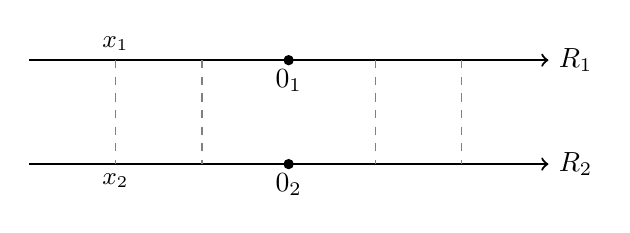
\begin{tikzpicture}[scale=1.1]
    % Recta R1
    \draw[thick, ->] (-3, 1.2) -- (3, 1.2) node[right] {$\mathbb{R}_1$};
    \filldraw (0, 1.2) circle (1.5pt) node[below] {$0_1$};
    
    % Recta R2
    \draw[thick, ->] (-3, 0) -- (3, 0) node[right] {$\mathbb{R}_2$};
    \filldraw (0, 0) circle (1.5pt) node[below] {$0_2$};

    % Líneas de identificación verticales (discontinuas)
    \draw[dashed, gray] (-2, 1.2) -- (-2, 0);
    \draw[dashed, gray] (-1, 1.2) -- (-1, 0);
    \draw[dashed, gray] (1, 1.2) -- (1, 0);
    \draw[dashed, gray] (2, 1.2) -- (2, 0);
    
    \node at (-2, 1.2) [above] {\small $x_1$};
    \node at (-2, 0) [below] {\small $x_2$};
\end{tikzpicture}
\end{center}

Sea $R$ la relación en $X$ definida por
\[x R y \text{ si }
\begin{cases}
x, y \in \mathbb{R}_1 \text{ ó } x, y \in \mathbb{R}_2 \text{ y } x = y \\[1ex]
x \in \mathbb{R}_1, y \in \mathbb{R}_2 \text{ (ó viceversa) y } x = y \in \mathbb{R} \setminus \{0\}
\end{cases} \text{}
\]
\textit{(El $0_1$ no lo identifica con $0_2$)}

\[
X \xrightarrow{\pi} \modulo{X}{R} = \text{ la recta real con el origen desdoblado (como espacio topológico)} 
\]

\begin{center}
\begin{tikzpicture}[scale=1.1]
    % Recta dividida antes del origen
    \draw[thick] (-3, 0) -- (-0.1, 0);
    % Parte derecha después del origen
    \draw[thick, ->] (0.1, 0) -- (3, 0) node[right] {$\mathbb{R}$};
    
    % Origen desdoblado (dos puntos superpuestos en la bifurcación)
    \filldraw[blue] (0, 0.3) circle (1.5pt) node[above] {$0_1$};
    \filldraw[red] (0, -0.3) circle (1.5pt) node[below] {$0_2$};
    
    % Conexiones sutiles hacia el origen desdoblado
    \draw[dashed, blue] (-0.3, 0) -- (0, 0.3) -- (0.3, 0);
    \draw[dashed, red] (-0.3, 0) -- (0, -0.3) -- (0.3, 0);
\end{tikzpicture}
\end{center}

Un subconjunto $W \subseteq \modulo{X}{R}$ es abierto si (es $\iff$):

\begin{enumerate}
    \item $0_1, 0_2 \notin W \implies \begin{array}{l} W \subseteq \mathbb{R}_1 \text{ es abierto} \\ W \subseteq \mathbb{R}_2 \end{array} \iff W \subseteq \mathbb{R} \text{ es abierto } \text{\small(en esta parte no ha cambiado nada)}$.

    \item $\begin{array}{l} 0_1 \in W \\ 0_2 \notin W \end{array} \implies \begin{array}{l} W \subseteq \mathbb{R}_1 \text{ es abierto} \\ W \setminus \{0_1\} \subseteq \mathbb{R}_2 \text{ es abierto} \end{array} \iff W \subseteq \mathbb{R} \text{ es abierto}$.

    \item Ídem para $\begin{array}{l} 0_2 \in W \\ 0_1 \notin W \end{array}$.

    \item $0_1, 0_2 \in W \implies \begin{array}{l} W \subseteq \mathbb{R}_1 \text{ es abierto} \\ W \subseteq \mathbb{R}_2 \end{array} \iff W \subseteq \mathbb{R} \text{ es abierto}$.
\end{enumerate}
\end{ejem}
\chapter{Espacios métricos y pseudométricos}
Sea $X$ un conjunto
\begin{defi} Una \textbf{pseudométrica} $d$ en $X$ es una aplicación de conjuntos
\[
    X \times X \overset{d}{\longrightarrow} \mathbb{R}
\]
verificando las propiedades
\begin{enumerate}
    \item $d(x, y) \ge 0, \, \forall x, y \in X \quad \text{y} \quad d(x, x) = 0, \, \forall x \in X$
    \item Simétrica $d(x, y) = d(y, x), \quad \forall x, y \in X$
    \item Desigualdad triangular $d(x, y) \le d(x, z) + d(z, y), \quad \forall x, y, z \in X$
\end{enumerate}
\end{defi}
\begin{defi} Una \textbf{métrica} ó \textbf{distancia} en $X$ es una pseudométrica $d$ que verifica que:
\[
    d(x, y) = 0 \iff x = y
\] \end{defi}
\begin{ejem} $\mathbb{R}^n$ como conjunto
\[
    d(x, y) = +\sqrt{\sum_{k=1}^n (x_k - y_k)^2} \quad \text{(se prueba que es una distancia)}
\]
donde $x = (x_1, \ldots, x_n) \in \mathbb{R}^n, y = (y_1, \ldots, y_n) \in \mathbb{R}^n$. Entonces $(\mathbb{R}^n, d)$ es un espacio métrico.

Definimos 
$$ \bt \overline{d} : \mathbb{R}^n \times \mathbb{R}^n \rar &  \mathbb{R} \\[-5mm] (x, y) \rarmaps & \overline{d}(x, y) &[-11mm] = \min\{1, d(x, y)\} \et $$
$\overline{d}$ es una métrica en $\mathbb{R}^n$ (se prueba). Es la \textbf{métrica acotada}.
\end{ejem}